\section{Background}

In this section, we briefly explain the concepts and technologies related to notification service in web and provide background of the two tools that are used majorly in our system. Recent changes in the development if HTML5 has created notable web features such as \texttt{Service Workers, Push Notifications} and \texttt{cache}. Any traditional website that adopts these features are known as Progressive Web Apps(PWAs). Using these features, it has become easier for the websites to cache web pages, provide offline loading, perform background processing and deliver push notifications. Earlier push notifications were only applicable to mobile applications. However, the new features lets any website to send a push notification to it's users from a browser used either in mobile or desktop. Throughout this paper, we refer to push notifications sent using a browser as Web Push Notifications(\textbf{WPN}) and Service Worker as just worker . We explain the two major web features involved in delivering WPNs, \texttt{Service Workers} and \texttt{Push Notifications}, cloud messaging service and the two tools that aids us in our implementation, JSGraph\ref{jsgraph} and Puppeteer\ref{puppeteer} as follows.


\begin{figure}[ht]
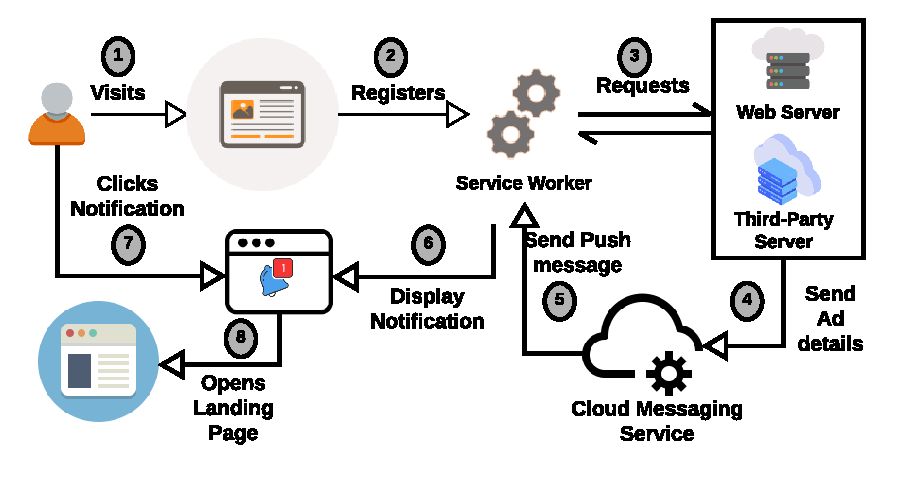
\includegraphics[width=\columnwidth]{figs/service_worker.pdf}
\caption{Steps involved in Serving Ads via WPNs}
\label{notification_system}
\end{figure}



\noindent \textbf{Service Workers and Push Notifications:} A Service Worker is basically a javascript file that runs in the background with a context different from a web page process. For a service worker to be installed and running, a user has to visit a web page that provides a link to the service worker javascript file. A service worker registers itself as long as the web page that it was downloaded to was served via HTTPS. A service worker plays multiple roles when it comes to different functionalities such as offline loading, background processing and pushing web notifications. Since this paper focuses on WPNs, we limit our explanation of service worker to it's role in WPNs. Once a service worker is registered, to subscribe to WPN, it needs to check if the website has permission from user to send notification. A subscription is made by exchanging keys that can be used to validate the sender and receiver of the push notifications. On visiting multiple Progressive Web Apps(WPA), multiple service workers gets registered on the device. Further, a single PWA is allowed to register multiple service workers as well. Therefore, the subscription helps create a mapping between the service worker and the ad server that is authorized to send notifications to it. After subscribing to WPNs, the role of service worker is to listen to any push messages sent for it to display and it does so by using a listener to \texttt{OnPush} event. At this point, service worker uses the \texttt{ShowNotification} event of \texttt{Notification} API to display the push message as a web notification. The notification has certain customizable parameters such as title, body, target URL, icon image, display image and action buttons. The user can then interact with the shown notification by either clicking on it, closing it or performing any custom actions that are shown in the notification. The service worker can choose to listen to any such user events and act accordingly. A service worker can make requests to fetch resources from any server or to send reports on the click events to any server. Usually, a service worker once registered will continue to exist in the user's machine unless they are explicitly unregistered. A step by step illustration of serving ads via WPNs is shown in Fig.\ref{notification_system}.   

\noindent \textbf{Firebase Cloud Messaging(FCM):} FCM is a cross-platform messaging solution for Web based Push Notifications. It serves as a central authority mediating the communications between the ad server and  the service worker. At the subscription stage, FCM creates a unique registration id per user per service worker and this is sent along with an endpoint to the ad server. Whenever an ad server wishes to send a notification to its subscribed user, it makes a request to FCM server along with the endpoint. FCM authenticates the sender using the keys that were exchanged earlier and it is using this endpoint that FCM understands which user machine and browser it has to deliver the notification. \warn{Should I explain the difference in receiving push messages between desktop and mobile here? It is explained later in system design}   

\noindent \textbf{JSGraph:} JSGraph by Bo Li et al. \ref{jsgraph} is a forensic engine that enables logging of  JavaScript(JS) executions and JS- driven DOM modifications within the browser at a fine-grained level. JSGraph is implemented by instrumenting Chromium code base and thus makes it portable to different platforms and browsers that support Blink/V8 engine. With the help of JSGraph, we can record all changes to the DOM, monitor navigation events, record execution details about Javascript code and changes to the DOM that are made by the Javascript code. Since Javascript plays a major role in advertising, we need a clear understanding of the scripts involved in advertisements and their effects. Any more changes required to suit our needs could be done by following a similar procedure of modifying Chromium code base. Moreover, the overhead caused by the instrumentation is acceptable thus making it a suitable tool for us to develop our system.

\noindent \textbf{Puppeteer:} Puppeteer is a NodeJS library that allows us to automatically control Chromium or Chrome over headless or non-headless mode. Since this is a tool developed by Google Chrome, it provides support to most features of Chromium and the code can be customized to suit our needs. This tool provides us with high level API useful to perform actions such as open window, navigate to a page,record network requests and responses, perform events such as click, scroll and select, capture screenshots and monitor multiple tabs. In our project, Puppeteer tool is also used to monitor events related to service workers and any requests made by the service worker. To achieve this, we found a service worker module of puppeteer that is still under development and use its features.

% With introduction of smart phones and development of their software development kits, very soon delivering information to the smart phone through push notifications became a dominant feature in apps. Push notifications allowed delivery of updates and content to apps in a resource aware manner. This meant the applications did not need to be always active draining power and processing resource, and yet, they were able to receive updates. 
% It was only recently that such long awaited feature was introduced for the web world as Web Push Notification-WPN-. Web push notifications in general contain three major components, a requester that provides the content, a relay server which receives the content and distributes them among the users and a subscriber code running on target devices which stands by -usually in the background- to receive the notifications. WPNs differ from push notifications delivered to mobile applications by the fact that WPNs do not require any installed code through the applications, they are cross platform and they are handled by the browsers not other applications. 

% In Google Chrome WPNs rely on \textit{service workers}. Service workers allow web sites to spin off a background process. once registered, this back ground process will stay active even when user is not interacting with the page directly and are majorly used for receiving WPN or syncing in the background. 
% To receive WPN in Google Chrome, a web site has to first be granted push notification permission, then it will launch a service worker and register the device with the push provider. Service worker will wait on new content to be delivered from push provider, then based on the content or the metadata in the pushed object then, service worker will decide its logic which might include showing a popup message or syncing and updating a piece of data. 




